\documentclass[]{article}
\usepackage{lmodern}
\usepackage{amssymb,amsmath}
\usepackage{ifxetex,ifluatex}
\usepackage{fixltx2e} % provides \textsubscript
\ifnum 0\ifxetex 1\fi\ifluatex 1\fi=0 % if pdftex
  \usepackage[T1]{fontenc}
  \usepackage[utf8]{inputenc}
\else % if luatex or xelatex
  \ifxetex
    \usepackage{mathspec}
  \else
    \usepackage{fontspec}
  \fi
  \defaultfontfeatures{Ligatures=TeX,Scale=MatchLowercase}
\fi
% use upquote if available, for straight quotes in verbatim environments
\IfFileExists{upquote.sty}{\usepackage{upquote}}{}
% use microtype if available
\IfFileExists{microtype.sty}{%
\usepackage{microtype}
\UseMicrotypeSet[protrusion]{basicmath} % disable protrusion for tt fonts
}{}
\usepackage[unicode=true]{hyperref}
\PassOptionsToPackage{usenames,dvipsnames}{color} % color is loaded by hyperref
\hypersetup{
            pdftitle={Master thesis},
            pdfauthor={Sylvain SCHMITT},
            colorlinks=true,
            linkcolor=Maroon,
            citecolor=Blue,
            urlcolor=Blue,
            breaklinks=true}
\urlstyle{same}  % don't use monospace font for urls
\usepackage{natbib}
\bibliographystyle{plainnat}
\usepackage{longtable,booktabs}
\usepackage{graphicx,grffile}
\makeatletter
\def\maxwidth{\ifdim\Gin@nat@width>\linewidth\linewidth\else\Gin@nat@width\fi}
\def\maxheight{\ifdim\Gin@nat@height>\textheight\textheight\else\Gin@nat@height\fi}
\makeatother
% Scale images if necessary, so that they will not overflow the page
% margins by default, and it is still possible to overwrite the defaults
% using explicit options in \includegraphics[width, height, ...]{}
\setkeys{Gin}{width=\maxwidth,height=\maxheight,keepaspectratio}
\IfFileExists{parskip.sty}{%
\usepackage{parskip}
}{% else
\setlength{\parindent}{0pt}
\setlength{\parskip}{6pt plus 2pt minus 1pt}
}
\setlength{\emergencystretch}{3em}  % prevent overfull lines
\providecommand{\tightlist}{%
  \setlength{\itemsep}{0pt}\setlength{\parskip}{0pt}}
\setcounter{secnumdepth}{5}
% Redefines (sub)paragraphs to behave more like sections
\ifx\paragraph\undefined\else
\let\oldparagraph\paragraph
\renewcommand{\paragraph}[1]{\oldparagraph{#1}\mbox{}}
\fi
\ifx\subparagraph\undefined\else
\let\oldsubparagraph\subparagraph
\renewcommand{\subparagraph}[1]{\oldsubparagraph{#1}\mbox{}}
\fi
\usepackage{booktabs}
\usepackage{amsthm}
\makeatletter
\def\thm@space@setup{%
  \thm@preskip=8pt plus 2pt minus 4pt
  \thm@postskip=\thm@preskip
}
\makeatother

\title{Master thesis}
\author{Sylvain SCHMITT}
\date{2017-06-01}

\usepackage{amsthm}
\newtheorem{theorem}{Theorem}[section]
\newtheorem{lemma}{Lemma}[section]
\theoremstyle{definition}
\newtheorem{definition}{Definition}[section]
\newtheorem{corollary}{Corollary}[section]
\newtheorem{proposition}{Proposition}[section]
\theoremstyle{definition}
\newtheorem{example}{Example}[section]
\theoremstyle{remark}
\newtheorem*{remark}{Remark}
\begin{document}
\maketitle

\thispagestyle{empty}
\begin{center}
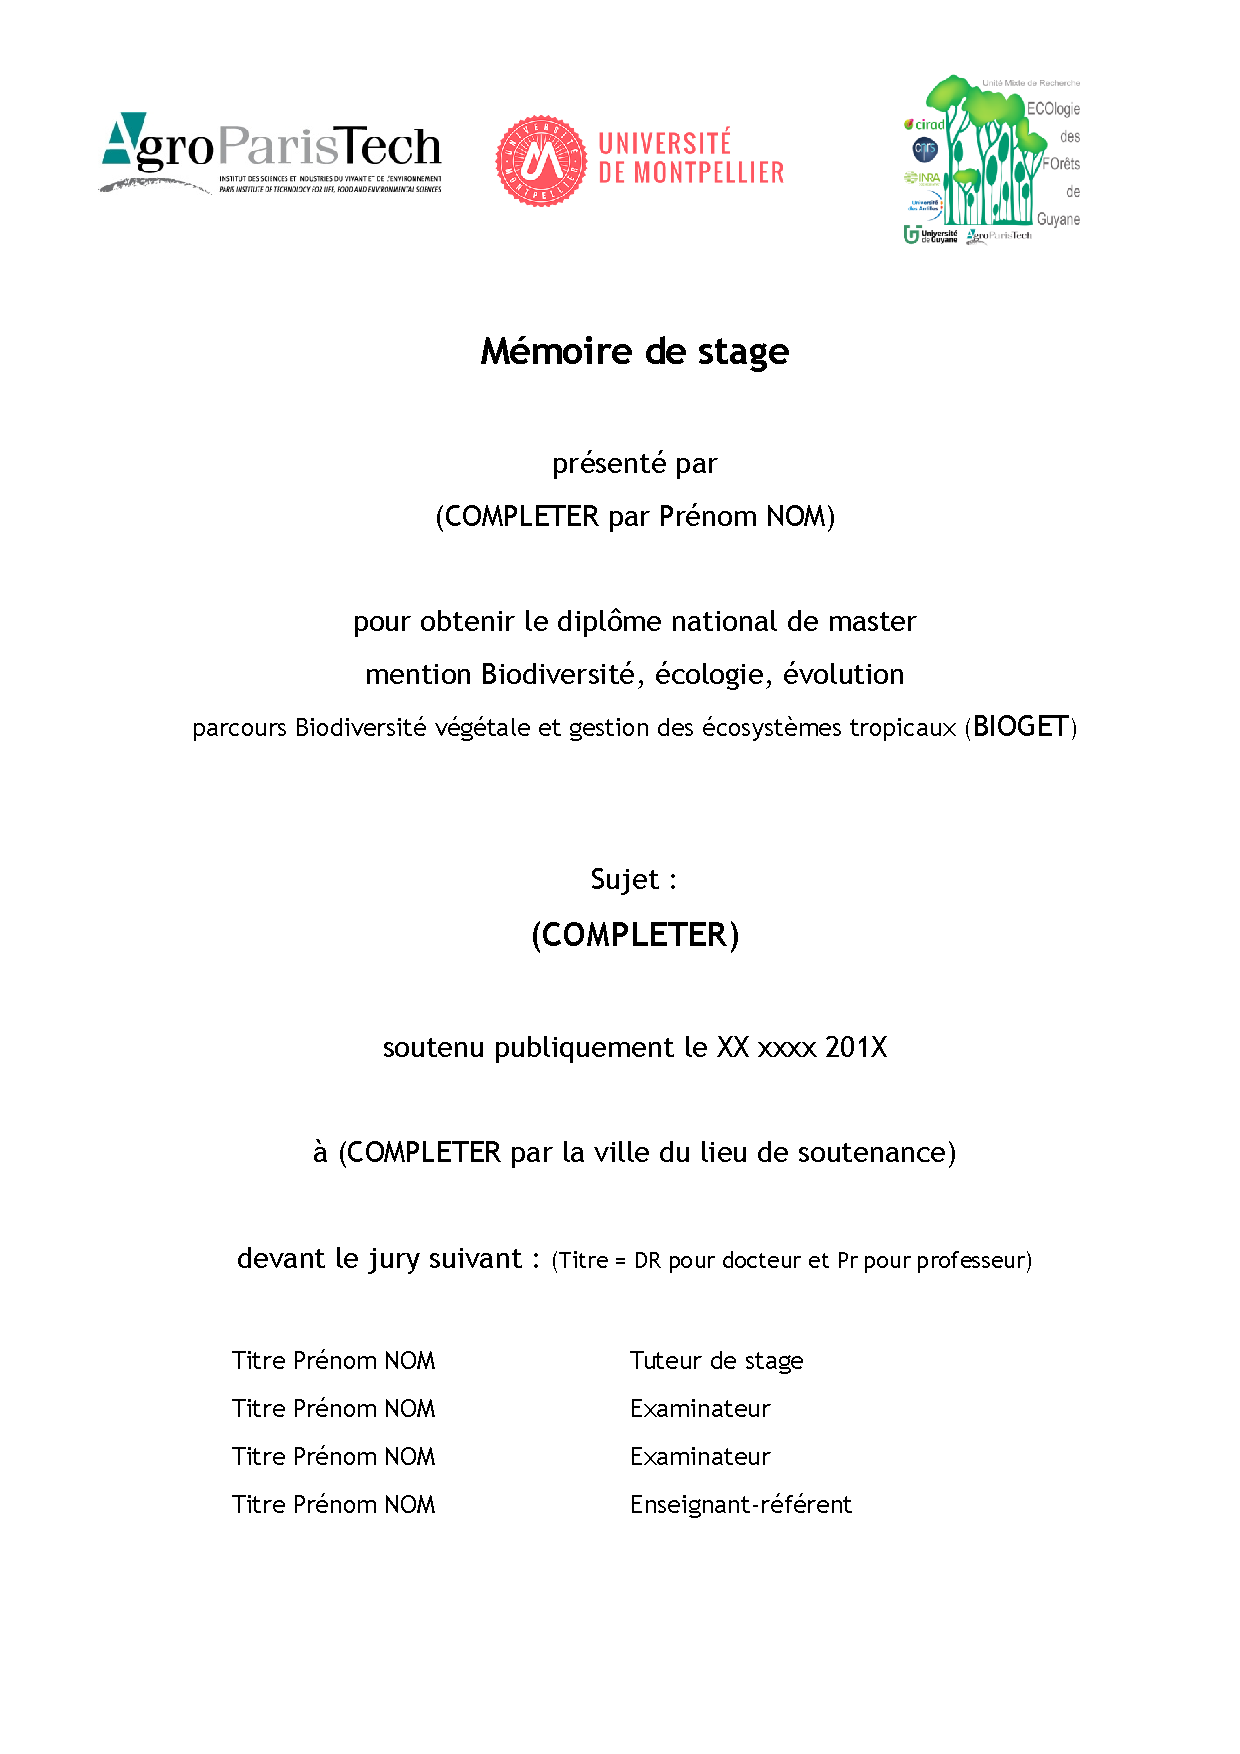
\includegraphics{images/main.pdf}
\end{center}

\setlength{\abovedisplayskip}{-5pt}
\setlength{\abovedisplayshortskip}{-5pt}

\thispagestyle{empty}
\begin{center}

\includegraphics{images/second.pdf}
\end{center}

\setlength{\abovedisplayskip}{-5pt}
\setlength{\abovedisplayshortskip}{-5pt}

{
\hypersetup{linkcolor=black}
\setcounter{tocdepth}{2}
\tableofcontents
}
\section*{Résumé et Abstract}\label{resume-et-abstract}
\addcontentsline{toc}{section}{Résumé et Abstract}

Écrire le résumé français ici\ldots{}

Write the english abstract here\ldots{}

\section*{Acknowledgments}\label{acknowledgments}
\addcontentsline{toc}{section}{Acknowledgments}

I would like to thank\ldots{}

\section*{Introduction}\label{introduction}
\addcontentsline{toc}{section}{Introduction}

Sutainable forest management in the tropics (i.e.~managed selective
harvesting of timber) has been widely promoted internationnaly to combat
tropical deforestation and degradation \citep{Zimmerman2012}. Currently
tropical logging accounts for one eight of global timber production
\citep{Blaser2011} and is still increasing. Most tropical timber
production originates from selective logging, the targeted harvesting of
timber from commercial species in a single cuttint cycle
\citep{Martin2015}.

On the other hand, tropical rainforests have fascinated ecologists due
to their outstanding diversity \citep{connell_diversity_1978}.
Effectively tropical forests host over half of the Earth's biodiversity
\citep{Scheffers2012}. High biodiversity from tropical rainforests is
the source of many ecosystem functions. Amongst others, tropical forests
play a key role in biogeochemical cycles, including carbone storage
\citep{Lewis2004}. \textbf{Add insights into carbon storage role of
tropical forest.} Ecosystem functions from tropical forests support
numerous ecosystem services, such as timber production and climate
regulation.

But several authors argue that selective logging represents a major
threat to biodiversity
\citep{Carreno-Rocabado2012, DeAvila2015, Gibson2013, Martin2015, Zimmerman2012},
challenging the sustainable definition from current selective logging.
We consequently need to assess both short and long term impacts of
selective logging on tropical forest ecosystems to implement better
syslvicultural practives in order to reach sustainability.

The question of selective logging impact on tropical forest can be
directly related to the emerging field of biodiversity and ecosystem
functionning \citep{Loreau2000}. Tropical forest outstanding
biodiversity will be both a factor and a result of forest ecosystem
response to logging disturbance. And forest ecosystem response to
logging disturbance will directly modify ecosystem functionning in both
short and long term. Consequently assessing selective logging effect on
tropical forest linking biodiversity and ecosystem seems an obvious and
promising way \citep{Loreau2010}. \textbf{Paragraph to fully review !}

Negative short term impacts of selective logging have been assessed
\citetext{\citealp{Carreno-Rocabado2012}; \citealp{DeAvila2015}; \citealp[but
see][]{Martin2015}}. Much less is known about the long term impact
\citep{Osazuwa-Peters2015}. The main reason is the difficulty to conduct
long term empirical study \citep[but see][]{Herault2010}, which can be
completed by the use of forest simulators
\citep{Huth2004, Khler2004, Ruger2008, Tietjen2006}. Individual-based
models of forest dynamics present the perfect framework to develop such
joint biodiversity-ecosystem approaches \citep{Li}. Individual-based
models describe forest `patches' accumulating carbon through time,
assessing tree growth within the patch, or releasing carbon through gap
opening \citep{Bugmann2001}. Up to several dozens of different Plant
Functional Types (PFTs) are generally defined and models can sometimes
be fully spatially explicit \citep{Pacala1996}. Recently, the forest
growth simulator TROLL \citep{Chave1999}, an individual-based and
spatially explicit forest model, was developped to introduce recent
advances in plant physiological community. TROLL model relates
physiological processes to species-specific functional traits
\citep{Li}. Consequently, TROLL model allow to simulate fully a
neotropical forest biodiversity to study biodiversity-ecosystem
functionning link response to logging disturbance.

\textbf{Major question greater diversity (taxonomic and functional)
brought a better resilience to disturbance ?}

\section{Model description}\label{model-description}

\subsection{Overview}\label{overview}

TROLL model each tree indivdually in a located environment. Thus TROLL
model, alongside with SORTIE \citep{Pacala1996, Uriarte2009} and FORMIND
\citep{Fischer2016, Kohler1998}, can be defined as an individual-based
and spatially explicit forest growth model. TROLL simulates the life
cycle of individual trees from recruitment, with a diameter at breast
height (dbh) above 1 cm, to death with growth and seed production. Trees
are growing in a located light environment explicitly computed witin
voxels of 1 \(m^3\). Each tree is consistently defined by its age,
diameter at brest height (dbh), height (h), crown radius (CR), crown
depth (CD) and leaf area (LA) (see figure \ref{fig:TROLLtree}). Tree
geometry is calculated with allometric equations but leaf area vary
dinamically within each crown following carbon allocations. Voxels
resolution of 1 \(m^3\) allow the establishment of maximum one tree by
1x1 m pixels. Each tree is flagged with a species label inherited from
the parent tree through the seedling recruitment. A species label is
associated to a number of species specific parameters (see table
\ref{tab:traits}) related to functional trait values which can be
sampled on the field.

\begin{table}

\caption{\label{tab:traits}Species-specific parameters used in TROLL from @Li. Data originates from the BRIDGE [@Baraloto2010] and TRY [@Kattge2011] datasets.}
\centering
\begin{tabular}[t]{l|l|l}
\hline
Abbreviation & Description & Units\\
\hline
\$LMA\$ & leaf mass per area & \$g.m\textasciicircum{}\{-2\}\$\\
\hline
\$N\_m\$ & leaf nitrogen content per dry mass & \$mg.g\textasciicircum{}\{-1\}\$\\
\hline
\$P\_m\$ & leaf phosphorous content per dry mass & \$mg.g\textasciicircum{}\{-1\}\$\\
\hline
\$wsg\$ & wood specific gravity & \$g.cm\textasciicircum{}\{-3\}\$\\
\hline
\$dbh\_\{thresh\}\$ & diameter at breasth height threshold & \$m\$\\
\hline
\$h\_\{lim\}\$ & asymptotic height & \$m\$\\
\hline
\$a\_h\$ & parameter of the tree-height-dbh allometry & \$m\$\\
\hline
\end{tabular}
\end{table}

Carbon assimilation is computed over half-hourly period of a
representative day. Then allocation is computed to simulate tree growth
from an explicit carbone balance (in contrast to previous models).
Finally environment is updated at each timestep set to one month.
Seedlings are not simulated explicitly but as a pool. In addition
belowground processes, herbaceous plants, epiphytes and lianas are not
simulated inside TROLL. The source code is written in C++ and available
upon request. All analyses were conducted in R version 3.4.0
\textbf{Cite R, add entry in Mendeley}.

\begin{figure}[htbp]
\centering
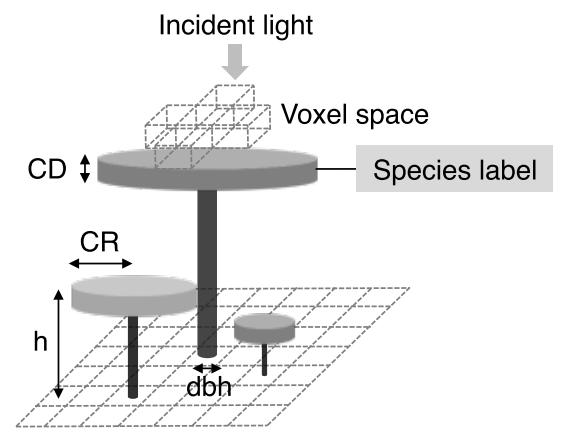
\includegraphics{images/TROLLtree.png}
\caption{\label{fig:TROLLtree}Individuals tree inside TROLL explicit spatial
grid from \citet{Li}. Tree geometry (crown radius CR, crown depth CD,
height h, diameter at breast height dbh) is updated at each timestep
following allometric relationship with assimilated carbon allocated to
growth. Each tree is flagged with a species label linking to its
species-specific attributes. Light is compputed explicitly at each
timestep for each voxel.}
\end{figure}

\subsection{Abiotic environment}\label{abiotic-environment}

A voxel space, with a resolution of 1 \(m^3\), is used to explicilty
model the abiotic environment. For each tree crown, leaf area density is
calculated on tree geometry assuming a uniform distriution across voxels
occupied by the crown. Leaf area density is computed within each voxel
summing all tree crowns inside the voxel \(v\), and is denoted
\(LAD(v)\) (leaf area per voxel in \(m².m^{-3}\)). The vertical sum of
\(LAD\) from voxel \(v\) to the ground level defines \(LAI(v)\) (leaf
area per fround area in \(m^2.m^{-2}\) commonly called leaf area index):

\begin{equation}
  LAI(v) = \sum _{v'=v} ^\infty LAD(v') 
  \label{eq:LAI}
\end{equation}

Daily variations in light intensity (photosynthetic photon flux density
PPFD in \(\mu mol_{photons}.m^{-2}.s^{-1}\)), temperature (T in degrees
Celsius), and vapor pressure deficit (VPD in \(kPA\)) are computed to
assess carbon assimilation within each voxel of the canopy and for a
representative day per month (see Appendix 1 from \citet{Li} for further
details). Variation of PPFD Within the canopy is calculated as a loacal
Beer-Lambert extinction law:

\begin{equation}
  PPFD_{max,month}(v) = PPFD_{top,max,month}*e^{-k*LAI(v)}
  \label{eq:PPFD}
\end{equation}

The daily maximum incident PPFD at the top of canopy
\(PPFD_{top,max,month}\) is given as input. The extinction rate \(k\) is
assumed as constant, besides is variation with zenith angle and species
leaf inclination angle \citep{Meir2000}. Moreover only vertical light
diffusion is considered ignoring lateral light diffusion, which can have
an important role especially in logging gaps. Finally, intra-day
variation at half hour time steps \(t\) for a representative day every
month are used to compute \(PPFD_{month}(v,t)\), \(T_{month}(v,t)\) and
\(VPD_{month}(v,t)\). Water and nutrient process both in soil and inside
trees are not simulated.

\subsection{Photosynthesis}\label{photosynthesis}

\subsubsection{Theory}\label{theory}

Troll simulates the carbon uptake of each individual with the Farquhar,
von Caemmerer and Berry model of C3 photosynthesis \citep{Farquhar1980}.
Gross carbon assimilation rate (\(A\) in
\(\mu mol~CO_2. m^{-2}.s^{-1}\)) will be the minimum of eiter Rubisco
activity (\(A_v\)) or RuBP generation (\(A_j\)):

\begin{equation}
  A=min(A_v, A_j)~|~A_v=V_{cmax}*\frac{c_i-\Gamma^*}{c_i+K_m}~;~A_j=\frac{J}{4}*\frac{c_i-\Gamma^*}{c_i+2*\Gamma^*}
  \label{eq:A}
\end{equation}

\(V_{cmax}\) is the maximum rate of carboxylation
(\(\mu mol~CO_2.m^{-2}.s^{-1}\)). \(c_i\) is the \(CO_2\) partial
pressure at carboxylation sites. \(\Gamma^*\) is the \(CO_2\)
compensation point in absence of dark respiration. \(K_m\) is the
apparent knietic constant of the Rubisco. And \(J\) is the electron
transport rate (\(\mu mol e^-.m^{-2}.s^{-1}\)). \(J\) depends on the
light intensity with \(PPFD\):

\begin{equation}
  J = \frac{1}{2*\theta}*[\alpha*PPFD+J_{max}-\sqrt{(\alpha*PPFD+J_{max})^2}-4*\theta*\alpha*PPFD*J_{max}]
  \label{eq:J}
\end{equation}

\(J_{max}\) is the maximal electron transport capacity
(\(\mu mol e^-.m^{-2}.s^{-1}\)). \(\theta\) is the curvature factor. And
\(\alpha\) is the apparent quantum yield to electron transport
(\(mole^-.mol~photons^{-1}\)).

Carbon assimilation by photosynthesis will then be limited by the
\(CO_2\) partial pressure at carboxylation sites. Stomata controls the
gas concentration at carboxylation sites throught stomatal transport:

\begin{equation}
  A = g_s*(c_a-c_i)
  \label{eq:Ag}
\end{equation}

\(g_s\) is the stomatal conductance to \(CO_2\)
(\(molCO_2.m^{-2}.s^{-1}\)). TROLL simulates stomatal conductance
\(g_s\) with the model from \citep{Medlyn2011}:

\begin{equation}
  g_s = g_0 + (1 + \frac{g_1}{\sqrt{VPD}})*\frac{A}{c_a}
  \label{eq:gs}
\end{equation}

\(g_0\) and \(g_1\) are parameters from the model. TROLL model assume
\(g_0 \approx 0\) (empirically tested and considered as reasonable).

\subsubsection{Parametrization}\label{parametrization}

Leaf traits can be used as proxy of photosynthesis, especially leaf
nutrient content which directly play a role in it
\citep{wright_worldwide_2004}. \citet{Domingues2010} suggested that
\(V_{cmac}\) and \(J_{max}\) were both limited by the leaf concentration
of nitrogen \(N\) and phosphorus \(P\) (\(mg.g^{-1}\)):

\begin{equation}
  log_{10} V_{cmax-M} = min( 
  \begin{array}{c} 
    -1.56+0.43*log_{10} N-0.37*log_{10} LMA \\
    -0.80+0.45*log_{10} P-0.25*log_{10} LMA 
  \end{array} 
  )
  \label{eq:VcmaxM}
\end{equation}

\begin{equation}
  log_{10} J_{max-M} = min(
  \begin{array}{c} 
    -1.50+0.41*log_{10} N-0.45*log_{10} LMA \\
    -0.74+0.44*log_{10} P-0.32*log_{10} LMA 
  \end{array}
  )
  \label{eq:JmaxM}
\end{equation}

\(V_{cmax-M}\) and \(J_{max-M}\) are the photosynthetic capacities at
\(25^\circ C\) of mature leaves per leaf dry mass (resp.
\(\mu mol CO_2.g^-1.s^{-1}\) and \(\mu mol e^-.g^{-1}.s^{-1}\)). \(LMA\)
is the leaf mass per are (\(g.cm^{-2}\)). \(V_{cmax}\) and \(J_{max}\)
are calculated by multiplying \(V_{cmax-M}\) and \(J_{max-M}\) by
\(LMA\). \(V_{cmax}\) and \(J_{max}\) variation with temperature are
caluclated with \citet{Bernacchi2003} (see Appendix 2 from \citet{Li}
for further details).

TROLL computes leaf carbon assimilation \(A_l\) combining equations from
\eqref{eq:A} to \eqref{eq:JmaxM} for each tree crown voxel within in each
crown layer \(l\):

\begin{equation}
  A_l = \frac{1}{n_v*t_M} * \sum_v  \sum^{t_M}_{t=1} A(PPFD_{month}(v,t),VPD_{month}(v,t),T_{month}(v,t))
  \label{eq:Al}
\end{equation}

\(PPFD_{month}(v,t)\), \(VPD_{month}(v,t)\) , and \(T_{month}(v,t)\) are
derived from microclimatic data. \(n_v\) is the number of voxels within
crown layer \(l\). And the sum is calculated over the \(t_M\)
half-hourly intervals \(t\) of a tipical day.

\subsection{Autotrophic respiration}\label{autotrophic-respiration}

A large fraction of plants carbon uptake is actually used for plant
maintenance and growth respiration. The autotrophic respiration can
represents up to 65\% of the gross primary productivity but varies
strongly among species, sites, and environnements.

TROLL uses \citet{Atkin2015} database of mature leaf dark respiration
and associated leaf traits to compute leaf maintenance respiration:

\begin{equation}
  R_{leaf-M} = 8.5431-0.1306*N-0.5670*P-0.0137*LMA+11.1*V_{cmax-M}+0.1876*N*P
  \label{eq:Rl}
\end{equation}

\(R_{leaf-M}\) si the dark respiration rate per leaf dry mass at a
temperaure of \(25^\circ C\) (\(nmolCO_2.g^{-1}.s^{-1}\)). The other
terms are in equations \eqref{eq:VcmaxM} and \eqref{eq:JmaxM}. TROLL assume
leaf respiration during day light to be 40\% of leaf dark respiration,
and computes total leaf respiration by accounting for the legnth of
daylight.

TROLL model stem respiration (\(R_{stem}\) in \(\mu molC.s^{-1}\)) with
a constant respiration rate per volume of sapwood:

\begin{equation}
  R_{stem} = 39.6*\pi*ST*(dbh-ST)*(h-CD)
  \label{eq:Rs}
\end{equation}

dbh, h, CD and ST are tree diameter at breast height, height, corwn
depth and sapwoond thickness, respectively (\(m\)). TROLL assumes
\(ST=0.04~m\) when \(dbh>30~cm\) and an increasing \(ST\) for lower
\(dbh\).

Finally, TROLL computes both fine root maintenance respiration, as half
of the leaf maintenance respiration. Whereas coarse root and branch
maintenance respiration is computed as half of the stem respiration. And
growth respiration (\(R_{growth}\)) is assumed to account for 25\% of
the gross primary productivity minus the sum of maintenance
respirations.

\subsection{Net carbon uptake}\label{net-carbon-uptake}

Net primary production of carbon for one individual \(NPP_{ind}\)
(\(gC\)) is computed by the balance between gross primary production
\(GPP_{ind}\) and respirations \(R\):

\begin{equation}
  NPP_{ind} = GPP_{ind} - R_{maintenance} - R_{growth}
  \label{eq:NPP}
\end{equation}

TROLL partitions individuals total leaf area \(LA\) into three pools for
different leaf age classes corresponding to different photosynthesis
efficiency (young, mature and old leaves with \(LA_{young}\),
\(LA_{mature}\), and \(LA_{old}\) respectivelly). Consequently we can
compute growth primary production for one individual as:

\begin{equation}
  GPP_{ind} = 189.3 * \Delta t * \sum _{l= \lfloor h-CD \rfloor +1} ^{\lfloor h \rfloor} [A_l] * (\frac{LA_{young}}{2} + LA_{mature} + \frac{LA_{old}}{2})
  \label{eq:GPP}
\end{equation}

h and CD are tree height and crown depth, repectivelly (\(m\)).
\(\lfloor x \rfloor\) is the rounding function. \(\Delta t\) is the
duration of a timestep (\(year\)).

Thus, TROLL can compute carbon allocation to wood into an increment of
stem volume \(\Delta V\) (\(m^3\)):

\begin{equation}
  \Delta V = 10^{-6} * \frac{f_{wood}*NPP_{ind}}{0.5*wsg}*Senesc(dbh)
  \label{eq:DeltaV}
\end{equation}

\(f_{wood}\) is the fixed fraction of NPP allocated to stem and
branches. \(wsg\) is the wood specific gravity (\(g.cm^{-3}\), see
\ref{tab:traits}). TROLL assume large trees less efficient to convert
NPP as growth by using a size-related growth decline with function
\(Senesc\) after a specific diameter at brest height threshold
\(dbh_{thresh}\):

\begin{equation}
  Senesc(dbh) = max(0;3-2*\frac{dbh}{dbh_{thresh}})
  \label{eq:Senesc}
\end{equation}

Finally, TROLL can compute carbon allocation to canopy with canopy NPP
fraction denoted \(f_{canopy}\) and decomposed into leaf, twig and fruit
production. Carbon allocation to leaf results in a new young leaf pool,
whereas other leaf pools are updated as follow:

\begin{equation}
  \begin{array}{c} \\
   \Delta LA_{young} = \frac{2*f_{leaves}*NPP_{ind}}{LMA}-\frac{LA_{young}}{\tau_{young}} \\
  \Delta LA_{mature} = \frac{LA_{young}}{\tau_{young}} - \frac{LA_{mature}}{\tau_{mature}}\\
  \Delta LA_{old} = \frac{LA_{mature}}{\tau_{mature}} - \frac{LA_{old}}{\tau_{old}}
  \end{array}
  \label{eq:DeltaLA}
\end{equation}

\(\tau_{young}\), \(\tau_{mature}\), and \(\tau_{old}\) are species
residence times in each leaf pools (\(years\)). The sum of residency
time thus defined the leaf lifespan
\(LL = \tau_{young} + \tau_{mature} + \tau_{old}\) (\(years\)).
\(\tau_{young}\) is set to one month and \(\tau_{mature}\) is set to a
third of leaf lifespan \(LL\). Previous implementation of TROLL model
used \citet{Reich1991a} allometry to infer leaf lifespan \(LL\) from
species leaf mass per area \(LMA\) \citep{Li}. But the use of the
allometrie from \citet{Reich1991a} with current implementation of the
TROLL model resulted in an underestimation of leaf lifespan for low LMA
species. Consequently in the following paragraph we suggest a new
allometry. Belowground carbon allocation is not simulated inside TROLL.

\subsection{Leaf lifespan}\label{leaf-lifespan}

The underestimation of leaf lifespan for low LMA species with the
allometry from \citet{Reich1991a} resulted in indivduals unealistic
early death from carbon starvation. We gathered data from
TRY\citep{Kattge2011}, DRYAD \citep{chave_towards_2009} and GLOPNET
\citep{wright_worldwide_2004} datasets. We used an out of the bag method
applied on a random forest to select variables with highest importance
to explain leaf lifespan. We thus selected leaf mass per are \(LMA\),
leaf nitrogen content \(N\) and wood specific gravity \(wsg\). We then
used a bayesian approach to test different models with growing level of
complexity. The model with the best tradeoff between complexity (number
of parameters), convergence, likelihood, and prediction quality (root
mean square error of prediction RMSEP) was kept. We selected following
model with a maximum likelihood of 13.6 and a RMSEP of 12 months:

\begin{equation}
  LL_{d} \sim \mathcal{logN}({\beta_1}_d*LMA - {\beta_2}_d*N*\beta_3*wsg, \sigma)
  \label{eq:LLb}
\end{equation}

Leaf lifespan \(LL\) follows a lognormal law with location infered from
leaf lifespan \(LMA\), nitrogen content \(N\) and wood specific gravity
\(wsg\) and a scale \(\sigma\). Each \({\beta_i}_d\) is following a
normal law located on \(\beta_i\) with a scale of \(\sigma_i\). All
\(\beta_i\), \(\sigma_i\), and \(\sigma\) are assumed without
presemption following a gamma law. \(d\) represents the dataset random
effects and encompass environmental and protocol variations. The
sampling of model \eqref{eq:LLb} resulted in the following allometry:

\begin{equation}
  LL = e^{0.017*LMA - 0.103*Nmass + 1.94*wsg}
  \label{eq:LL}
\end{equation}

\subsection{Tree growth}\label{tree-growth}

Once the increment of stem volume \(\Delta V\) calculated with equation
\eqref{eq:DeltaV}, TROLL convert it into an increment of tree diameter at
breast height denoted \(\Delta dbh\). TROLL infer tree height from
\(dbh\) using a Michaelis-Menten equation:

\begin{equation}
  h = h_{lim}*\frac{dbh}{dbh + a_h}
  \label{eq:h}
\end{equation}

On the other hand, we have the trunk volume
\(V = C * \pi * (\frac{dbh}{2})^2*h\), thus:

\begin{equation}
  \begin{array}{c} \\
    \Delta V = C*\frac{1}{2}*\pi*h*dbh*\Delta dbh + C * \pi * (\frac{dbh}{2})^2*h \\
    \Delta V = V*\frac{\Delta dbh}{dbh}*(3-\frac{dbh}{dbh + ah})
  \end{array}
  \label{eq:Deltadbh}
\end{equation}

Next, TROLL used the new trunk dimension (\(dbh\) and \(h\)) to update
tree crown geometry using allometric equations \citep{Chave2005}:

\begin{equation}
  \begin{array}{c} \\
    CR = 0.80 + 10.47*dbh - 3.33*dbh^2\\
    CD = -0.48 + 0.26*h~;~CD = 0.13 + 0.17*h~(h<5~m)
  \end{array}
  \label{eq:C}
\end{equation}

Finally, TROLL computes the mean leaf density within the crown (\(LD\)
in \(m^2.m^{-3}\)) assuming a uniform distribution:

\begin{equation}
  LD = \frac{LA_{young}+LA_{mature}+LA_{old}}{\pi*CR^2*CD}
  \label{eq:LD}
\end{equation}

\subsection{Mortality}\label{mortality}

Mortality is partitioned in three factors inside TROLL: background death
\(d_b\), treefall death \(d_t\) and negative density dependent death
\(d_{NDD}\). Because density dependent death \(d_{NDD}\) is still in
development inside TROLL we did not used it, so we will not detail is
computation.

\citet{chave_towards_2009} advocated for a wood economics spectrum
opposing fast growing light wood species species with high risk of
mortality to slow growing dense wood species with reduced risk of
mortality. Hence, background mortality is derived from wood specific
gravity \(wsg\) inside TROLL:

\begin{equation}
  d_b = m*(1-\frac{wsg}{wsg_{lim}})+d_n
  \label{eq:db}
\end{equation}

\(m\) (\(events.year^{-1}\)) is the reference background death rate for
lighter wood species (pioneers). \(d_n\) represents death by
carbohydrates shortage. If the number of consecutive day with
\(NPP_{ind} < 0\) \eqref{eq:NPP} is superior to tree leaf lifespan \(d_n\)
is set to 1 and remains null in other cases.

Mortality by treefall inside TROLL depends on a specifric stochastic
threshold \(\theta\):

\begin{equation}
  \theta = h_{max}*(1-v_T*|\zeta|)
  \label{eq:theta}
\end{equation}

\(h_{max}\) is the maximal tree height. \(v_T\) is the variance term set
to 0.3. \(|\zeta|\) is the absolute value of a random centered and
scaled Gaussian. If the tree hieght \(h\) is superior to \(\theta\) then
the tree may fall with a probability \(1-\theta/h\) \citep{Chave1999}.
The treefall direction is random (drawn from a uniform law
(\(\mathcal{U}[0,2\pi]\)). All tree in the trajectory of the falling
tree will be hurted through a variable denoted \(hurt\), incremented by
fallen tree height \(h\). If a tree height is inferior than its \(hurt\)
values then it may die with a probability
\(1-\frac{1}{2}\frac{h}{hurt}\). \(hurt\) variable is reset to null at
each timestep (\(month\)).

\subsection{Recruitment}\label{recruitment}

Once the tree became fertile they will start to disperse seeds. TROLL
consider tree as fertile after a specific height threshold
\(h_{mature}\) \citep{Wright2005}:

\begin{equation}
  h_{mature} = -11.47+0.90*h_{max}
  \label{eq:hmature}
\end{equation}

But TROLL is not considering seed directly through a seedbank, instead
seed might be interpreted as a seedling recruitment opportunity. The
number of reproduction opportunities per mature tree is denoted \(n_s\)
and set to 10 for all species. This assumption originates from a
trade-off between seed number and seed size resulting in equivalent
survival and recruitment probability. All \(n_s\) events are dispersed
with a distance randomly drawn from a Gaussian distribution.
Additionally, TROLL model consider external seedrain through \(n_{ext}\)
events of seed immigration:

\begin{equation}
  n_{ext} = N_{tot}*f_{reg}*n_{ha}
  \label{eq:next}
\end{equation}

N\_\{tot\} is the external seedrain per hectare (number of reproduction
opportunities). \(f_{reg}\) is the species regional frequency.
\(n_{ha}\) is the simulated plot size in \(ha\).

Finally, a bank of seedlings to be recruited is defined for each pixel.
If the ground-level light reaches a species light compensation point
\(LCP\) the species will be recruited:

\begin{equation}
  LCP = \frac{R_{leaf}}{\phi}
  \label{eq:LCP}
\end{equation}

\(R_{leaf}\) is the leaf respiration for maintenance (see \eqref{eq:Rl}).
\(\phi\) is the quantum yield (\(\mu mol C.\mu mol~photon\)) set to
0.06. If several species reach their \(LCP\), one is picked at random.
Seedlings are recruited with following intial geometry:

\begin{equation}
  \begin{array}{c} \\
    dbh = \frac{a_h}{h_{max} - 1}\\
    h = 1~m\\
    CR = 0.5~m\\
    CD = 0.3~m\\
    LD = 0.8~m^2.^{-3}
  \end{array}
  \label{eq:C}
\end{equation}

\section{Sensitivity analysis}\label{sensitivity-analysis}

\citet{Li} already assessed TROLL model sensitivity to several
parameters (\(k\) see \eqref{eq:PPFD}, \(\phi\) see \eqref{eq:LCP}, \(g1\)
see \eqref{eq:gs}, \(f_{wood}\) see \eqref{eq:DeltaV}, \(f_{canopy}\) see
\eqref{eq:DeltaLA} and \(m\) see \eqref{eq:db}) which they assumed having a
key role in model functioning.

On the other hand, we decided to use TROLL to study resistance and
resilience of ecosystem face to disturbance, highlighting the role of
biodiversit. Consequently we particulrarly needed to assess the
importance of functional traits to further better control and evaluate
functional diversities. We also needed to assess the sensitivity of
TROLL model to the seed rain constant (\(n_{ext}\), see \eqref{eq:next})
because we assume it is one of the main factor of tree recruitments
after disturbance in simulations.

\subsection{Functional traits}\label{functional-traits}

TROLL model currenty uses leaf mass per area (\(LMA\) in \(g.m^{-2}\)),
leaf nitrogen content per dry mass (\(N_m\) in \(mg.g^{-1}\)), leaf
phosphorus content per dry mass (\(P_m\) in \(mg.g^{-1}\)), wood
specific gravity (\(wsg\) in \(g.cm^{-3}\)), diameter at breasth height
threshold (\(dbh_{thresh}\) in \(m\)), asymptotic height (\(h_{lim}\) in
\(m\)), and parameter of the tree-height-dbh allometry (\(a_h\) in
\(m\)). To assess the sensitivity of TROLL model to species functionnal
traits, we performed a sensitivity analysis by fixing species trait
values to their mean. Each trait was tested independently. We reduce to
a common mean traits with a Perason's correlation value \(r \geq 0.8\)
(\(h_{max}\) and \(a_h\) with a correlation of \(r=0.98\)).

\subsection{Seed rain}\label{seed-rain}

To assess the sensitivity of TROLL model to seed rain, we performed a
sensitivity analysis by fixing simulations seed rain constant to 2, 20,
200 and 2000 seeds per hectare (default value being 200 seeds per
hectare).

Simulations were conducted on Intel Xeon(R) with 32 CPUs of 2.00GHz and
188.9 GB of memory. We assumed maturity of the forest after 500 years of
regeneration (Maréchaux \& Chave) and computed simulation 100 years
after a disturbance event with 40\% loss of basal area. Due to computer
limitations we did not run replicate (besides it should be necessary to
reduce simulation stochasticity). To assess ecosystem outputs
sensitivity to studied parameters, we compared it to 100 replicates of
control simulations with all parameters set to default values. Ecosystem
outputs outside of the range of the control replicates values are
significantly influenced by the studied parameter.

\section{Disturbance}\label{disturbance}

Most tropical timber production originates from selective logging, the
targeted harvesting of timber from species of interest. Consequently,
tropical sylviculture can be assimilated to a disturbance. The main
difference between a disturbance and selective logging is the targetting
of both species and individuals of interest. So we decided to first
asses unselective disturbance effect on tropical forest ecosystem to
subsequently better understand selective logging effect.

We first implemented a disturbance module inside TROLL model to simulate
unselective disturbance. 60 tree communities were then defined with
different levels of both specific and functional richness to explore the
role of biodiversity on tropical forest ecosystem answer to disturbance.
Next, different levels of disturbance were simulated on previous mature
communities. Finally, resilience of ecosystem major global variables
(related to carbon stock, forest dynamic and florisitic structure) from
simulations were partitioned between selection effects and niche
complementarity \citep{Loreau2001}.

\subsection{Model description}\label{model-description-1}

Disturbance module was designed in the simplest way in order to relate
the ecosystem answer to volume lost without any individuals nor species
targetting. For a given iteration \(disturb_{iter}\), individuals are
picked randomly with a uniform law on the number of trees. Selected
individuals are then removed without trigerring a treefall to avoid any
side effect. The operation is repeated untill the disturbance result in
a defined lost basal area (\(disturb_{intensity}\) in \% of BA).

\subsection{Design of experiment}\label{design-of-experiment}

In order to assess the role of biodiversity in ecosystem answer to
disturbance, we needed to create a space of experiments encompassing
both variation of disturbance, biodiversity and time. Disturbance was
represented by percentage of basal area loss (0\%, 25\%, 50\% and 75\%).
Biodiversity was integrated with two components specific and functional
diversities. We used species richness \(SR\) to represents species
diversity (5, 25, and 125). Functional diversity can be related to
numerous components, and \citet{Borgy2017} argued for 5: richness,
divergence, regularity, overlap and mean. Because mature forest were
created from a bare soil with TROLL simulations, we could not control a
priori divergence, regularity and overlap but only assess theim before
diturbance. Consequently, we focused on functional richness with convex
hull volume \(CHV\) and functional mean with community weighted mean
\(CWM\). For each level of species richness \(SR\), we selected 20
communities with growing convex hull volume \(CHV\) but with a community
weighted means close to the regional species pool community weighted
means. Effectivelly, we did not wanted drastic change in community means
that could have more effect than functional richness itself. This design
of experiments resulted in 60 communities (\(5~SR*20~CHV\)) and 240
simulations (\(60 ~communities*4~levels~of~disturbance\)) over 600 years
(maturity being assumed after 500 years of regeneration \citep{Li}).
Figure \ref{fig:DOE} presents the design of experiment for communities
biodiversity after the forest mature were simulated, and thus before
disturbance. We obtained a broad range of both functionl dispersion
\(FDis\) and aboveground biomass \(AGB\) for simulated forest ecosystems
before disturbance.

\begin{figure}[htbp]
\centering
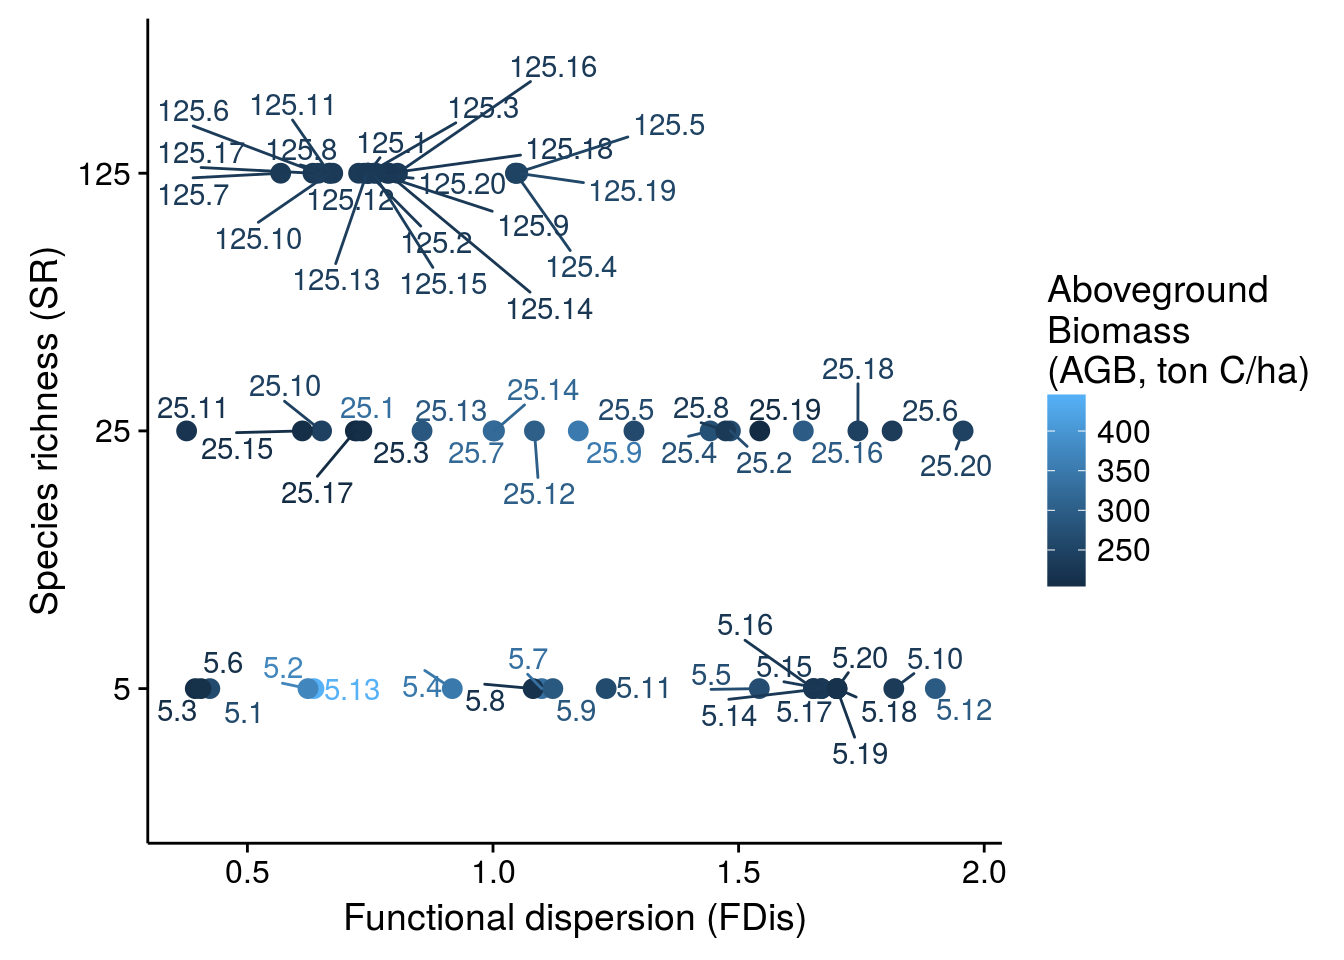
\includegraphics{master-thesis_files/figure-latex/DOE-1.pdf}
\caption{\label{fig:DOE}Experimental design before disturbance. Communities
are implemented along a gradient of species richness (SR) and functional
dispersion (FDis) resulting in a broad range of aboveground biomass
(AGB). FDis was caluclated based on 4 functional traits (leaf mass per
area, wood specific gravity, maximum diameter, maximum height).}
\end{figure}

\subsection{Ecosystem answer anlaysis}\label{ecosystem-answer-anlaysis}

Tropical forest ecosystems provides numerous ecosystem services linked
to several ecosystem functions. We focused on few functions and related
metrics to analyse ecosystem answer to disturbance: carbon stock with
aboveground biomass (\(AGB\) in \(ton~C.ha^{-1}\)), forest dynamic with
number of stem above \(10~cm\) diameter at breast height (\(N10\)), and
floristic composition with \textbf{?} (\textbf{?} in \textbf{?}).

The resilience of metrics values post disturbance were assessed through
\citet{Henry2012} formula:

\begin{equation}
  R\left(t\right)=\frac{Recovery\left(t\right)}{Loss\left(t_d\right)} \approx \frac{X(t)}{X(t_d-1)}
  \label{eq:Resilience}
\end{equation}

The resilience of the system \(R(t)\) at the time \(t\) is described by
the ratio of recovery \(Recovery(t)\) at time \(t\) to loss suffered
\(Loss(t_d)\) at disturbance time \(t_d\). We transformed the equation
in the resilience of the system \(R(t)\) at the time \(t\) being the
ratio of the ecosystem metric \(X(t)\) at time \(t\) to the ecosystem
metric before the disturbance happened \(X(t_d-1)\) at time \(t_d-1\).
\(X(t_d-1)\) was calculated as the mean of the ecosystem output for 50
last years of the simulation of the mature forest (over 600 years).
Then, we calculated for each simulation the recovery time
\(t_{recovery}\) were the ecosystem reached back its stable state
defined as its state before disturbance. But some ecosystem metrics can
reach pre disturbance value wihtout revealing ecosystem recovery. For
instance, number of stem above \(10~cm\) diameter at breast height
\(N10\) will first decrease due to disturbance. Then \(N10\) will exceed
its initial value due to new seedlings recruitment before decreasing
towards its pre disturbanec value. Consequently, the first time \(N10\)
reaches back its pre disturbance value can not be considered as the
recovery time \(t_{recovery}\). In order to solve this issue, we
considered the ecosystem as stable again when its whole set of observed
metrics reach their pre disturbance values.

Biodiversity is not only a facet of the experimental design and an
ecosystem output through florisitic composition, but also interact on
ecosystem functioning and consequently on its answer to disturbance.
Biodiversity ecosystem functioning relation can be split in
complementarity and selection effect with \citet{Loreau2001}
partitioning:

\begin{equation}
  \begin{array}{c}
    NE = X_O - X_E = CE + SE \\
    CE = N* \overline{\Delta RX} \overline{M}\\
    SE = N*cov(\Delta RX,M)
  \end{array}
  \label{eq:BiodivPart}
\end{equation}

Biodiversity net effect \(NE\) is based on the difference between
ecosystem variable \(X\) observed value \(X_O\) within the community
mixture of species and its expected value \(X_E\) if species performance
were equal to their performance in monocultures. This effect can be
partitioned between complementarity effect \(CE\), representing niche
partitionning, positive interactions, and resource supply, and selectvie
effect \(SE\) due to dominant species pool driving the ecosystem. Both
metrics depend on the variation of relative ecosystem variable
\(\Delta RX\):

\begin{equation}
  \Delta RX_{sp} = \frac{X_{sp}(mixture)}{X_{sp}(monoculture)} - P_{sp}
  \label{eq:DeltaRY}
\end{equation}

\(X_sp\) is the ecosystem variable value for one species either in
mixture \(X_{sp}(mixture)\) or in monoculture \(X_{sp}(monoculture)\).
\(P_{sp}\) is the proportion of the species in the mixture represented
by species relative abundance. Consequently, \(CE\) averages diversity
effects of all species presents in the mixture (both negatives and
positives). Whereas \(SE\) become positive when dominant species
outperform theimselves in mixture than in monoculture, and negative when
less dominant species outperform theimselves in mixture than in
monoculture \citep{Tobner2016}.

Recovery trajectories of ecosystem variable after disturbance were
partitioned between complementarity effect \(CE\) and selection effect
\(SE\). In order to do that, the design of experiment was repeated for
each species indivdually representing 652 simulations of monoculture.

\section{Selective logging}\label{selective-logging}

\subsection{Model description}\label{model-description-2}

\subsubsection{Designation}\label{designation}

\subsubsection{Selection}\label{selection}

\subsubsection{Rotten trees}\label{rotten-trees}

\subsubsection{Felling}\label{felling}

\subsubsection{Tracks}\label{tracks}

\subsubsection{Gap damages}\label{gap-damages}

\subsection{Design of experiment}\label{design-of-experiment-1}

\subsection{Outputs analysis ?}\label{outputs-analysis}

\subsubsection{Resistance and resilience
metrics}\label{resistance-and-resilience-metrics}

\subsubsection{Biodiversity
partitioning}\label{biodiversity-partitioning}

\section{Results}\label{results}

\subsection{Sensitivity}\label{sensitivity}

\subsection{Disturbance}\label{disturbance-1}

\subsection{Sylviculture}\label{sylviculture}

\section{Discussion}\label{discussion}

\bibliography{/home/sylvain/Documents/Bibliography/library.bib}

\end{document}
